\documentclass{report}
\usepackage[a4paper]{geometry}
\usepackage{ae,lmodern} 
\usepackage[francais]{babel}
\usepackage[utf8]{inputenc}
\usepackage[T1]{fontenc}
\usepackage{graphicx}
\usepackage{pdfpages}
\usepackage{lipsum}
\usepackage{listings}
\usepackage{titlesec}
\usepackage{pdfpages}
\usepackage{mwe}
\usepackage{lmodern}
\usepackage{graphicx} %%For loading graphic files
\usepackage{fancyhdr} %%definition perso d'en-têtes et pieds
\usepackage{amsmath}
\usepackage[linesnumbered,ruled]{algorithm2e}

\pagestyle{fancy}

\fancyhf{}
\setlength{\headwidth}{15cm}
\setlength{\headheight}{2cm}
\voffset 1pt


\renewcommand{\headrulewidth}{1pt}
\renewcommand{\footrulewidth}{1pt}
\fancyfoot[C]{\thepage}


\fancyhead[L]{
\includegraphics[scale=0.2]{ressources/p8.png}}

\titleformat{\chapter}[display]
  {\normalfont\bfseries}{}{0pt}{\Huge}

\titleformat{\section}[display]
  {\normalfont\bfseries}{}{0pt}{\Large}

\lstset{
numbers=left, 
numberstyle=\small, 
numbersep=8pt, 
frame = single, 
language=C, 
framexleftmargin=15pt}


\begin{document}




\begin{figure}
    \centering
    
\includegraphics[width=8cm]{ressources/p8.png}
    \title{Rapport : Projet Cryptographie \\ -- \\ Implantation de l’attaque par le milieu contre un chiffrement
    par bloc }
    \author{Thomas Roglin \\  }
    \date{26/12/2021}
    
    
\end{figure}


\maketitle

\newpage

\tableofcontents

\chapter{Introduction}
\paragraph{} 
Le but de ce projet est double. Il consiste tout d'abord en l'implémentation d'une version affaiblie de l'algorithme de chiffrement par bloc PRESENT, 
et appelé PRESENT24 pour sa version à 10 tours chiffrant des blocs de 24 bits.
Le second objectif de ce projet est d'implémenter une attaque par le milieu sur un message de 24 bits doublement chiffré.

\chapter{PRESENT}  
\section{ Présentation } 
PRESENT est algorithme de chiffrement par bloc conçu en 2007 par Bogdanov et al. et est notable pour sa faible taille, idéale pour une implémentation hardware. 
Il peut chiffrer des blocs de 64bits en utilisant une clef de taille 80 ou 128 bits.

PRESENT appartient à la famille des chiffrements dits SPN (Substitution-Permutation Network). Le principe
d’un chiffrement SPN est simple : chaque tour du chiffrement est constitué de trois couches :
\begin{itemize}
    \item Une addition (XOR) de la sous-clé du tour à l’état ;
    \item une couche de substitution pour assurer la confusion ;
    \item une couche linéaire pour assurer la diffusion.
\end{itemize}

La clef maitresse de l'algorithme sert à générer n sous clefs pour n tours grace à un algorithme de cadencement de clef.

\begin{algorithm}
    \SetKwInOut{Input}{Input}
    \SetKwInOut{Output}{Output}

    
    \Input{Un message de 64 bits $m$ et une clef maitre $key$ }
    \Output{Un chiffré de 64 bits $enc$}

    $state$ = $m$\;
    $K$ = generateRoundKeys($key$)\;
    \For{$i=1$ \KwTo $31$ }
      {
        $state$ = addRoundKey($state$,$Ki$)\;
        $state$ = sBoxLayer($state$)\;
        $state$ = pLayer($state$)\;
      }
      $enc$ = addRoundKey($state$,$K32$)\;
    \caption{Fonction de chiffrement d'un bloc de 64 bits par l'algorithme PRESENT}
\end{algorithm}

\paragraph{} Pour implémenter l'attaque, on utilisera une version de PRESENT affaiblie: PRESENT24. 
Elle chiffre des messages de 24bits, avec des clefs de 24 bits et en seulement 10 tours au lieu de 32.
Cependant, l'algorithme de cadencement des clefs sera repris du cadencement de PRESENT80 

\chapter{Attaque par le milieu }
\section{ 2PRESENT24 } 
\paragraph{} A l'instar de DoucleDES on considère le chiffremenent double 2PRESENT24. Ce chiffrement par bloc
prend en entrée deux clés $k1$ et $k2$ et chiffre un message $m$ de 24 bits une première fois avec PRESENT24
en utilisant la clé $k1$ et ensuite il chiffre le résultat une deuxième fois avec le même chiffrement mais avec
la clé $k2$, pour produire le chiffré $c$ :

\[ c  = 2PRESENT24 _{ k1,k2 }  (m) = PRESENT24_{ k2 }( PRESENT24_{ k1 }(m)) \] 

\section{ Principe de l'attaque  } 
\paragraph{} Pour mener à bien cette attaque, il est nécessaire de posséder aux minimums deux couples clairs chiffré 
$(m_{1},c_{1} )$ et $(m_{2},c_{2} )$ produits avec une clef secrète $(k_{1},k_{2})$. 
Cela fait donc de cette attaque, une attaque KPA: known-plaintext attack.

\paragraph{} Le but de cette attaque est de tester toutes les clefs possibles afin de retrouver la bonne paire de clef secrète.
Cependant, même si la clef est codé sur seulement $2^{24}$ bits, tenter toutes les $k_{1}$ possibles sur $m_{1}$ pour trouver $2^{24}$ messages chiffrés, 
puis retenter toute les $k_{2}$ pour trouver $2^{48}$ chiffrés dont un serait $c_{1}$ n'est pas envisageable. 
En effet une complexité de $2^{48}$ serait beaucoup trop grande.
 
\paragraph{} Cependant il est possible de diminuer la complexité en implémentant une attaque pour le milieu. 
Pour cela, on va commencer par chiffrer $m_{1}$ et $m_{2}$ avec les  $2^{24}$ $k_{1}$ clefs possibles, et stocker les chiffrés dans un grand tableau.
Puis, on va déchiffrer $c_{1}$ et $c_{2}$ avec les  $2^{24}$ $k_{2}$ clefs possibles, et stocker les déchiffrer  dans un deuxieme tableau.
Il suffit ensuite de comparer les 2 tableaux et de trouver l'élément commun pour trouver la paire de clef.

\newpage
\section{ pseudo code } 


\begin{algorithm}
    \SetKwInOut{Input}{Input}
    \SetKwInOut{Output}{Output}

    
    \Input{2 couples d'un message et de son chiffré de $2^{24}$ bits, $(m_{1},c_{1} )$ et $(m_{2},c_{2} )$ }
    \Output{2 clefs secretes $(k_{1},k_{2} )$ ayant permis de chiffrer les messages donnés en parametre   }

    $enc_msgs$ et $dec_keys$, deux tableaux de taille $2^{24}$ associant une clef à 2 chiffrés $k->(m_{1}, m_{2})$ \;

    \For{$key=0x0$ \KwTo $0xffffff$ }
      {
        $K$ = generateRoundKeys($key$)\;
        $enc\_msgs_{key}$ = (chiffre($m_{1}$, $K$), chiffre($m_{2}$, $K$)) \;
        $dec\_msgs_{key}$ = (dechiffre($c_{1}$, $K$), dechiffre($c_{2}$, $K$)) \;
      }
      \;
    sort($enc_msgs$)\;
    sort($dec_msgs$)\;
      \;
    \For{$key=0x0$ \KwTo $0xffffff$ }
    {
        $(m_1, m_2)$ = $enc\_msgs_{key}$\;
        \If{ $(k_{1},k_{2} )$ = search($(m_1, m_2)$, $dec\_msgs$) }{
            return $(k_{1},k_{2} )$\;
        }
    
    }


    \caption{Fonction principale de l'attaque par le milieu contre 2PRESENT24 }
\end{algorithm}



\chapter{Optimisation}
\section{ Substitution } 

\begin{lstlisting}
    u8_t subsitution_8(u8_t m) {
        u8_t sbox[16] =
          {0xc,0x5,0x6,0xb,0x9,0x0,0xa,0xd,
           0x3,0xe,0xf,0x8,0x4,0x7,0x1,0x2 };
        
        return (sbox[(m & 0xf0)>>4]<<4) | sbox[(m & 0x0f)];
    }
\end{lstlisting}

\begin{lstlisting}
    u32_t subsitution_24( u32_t m ){
        static const u32_t sbox[16] = {
            12,5,6,11,9,0,10,13,3,14,15,8,4,7,1,2
        };

        u32_t m2 = 0;
        for(int i = 5; i >= 0; i-- ){
            m2 = m2 << 4 ;
            m2 = m2 | sbox[ 15 & ( m >> ( i * 4 ) ) ];
        }
        return m2;

    }
\end{lstlisting}

\paragraph{} Ces deux fonctions de substitution sont très similaires, 
cependant la première prend un message de 8 bits et renvoie directement un message de 8 bits avec les 4 premiers et dernier bit passés dans la Sbox.
La deuxième fonction prend un message m1 de 24bits et va construire un message m2 de 24 bits en décalant 4 bits par 4 bits tout en ajoutant ajoutant 4 bits de m1 passé dans la Sbox.

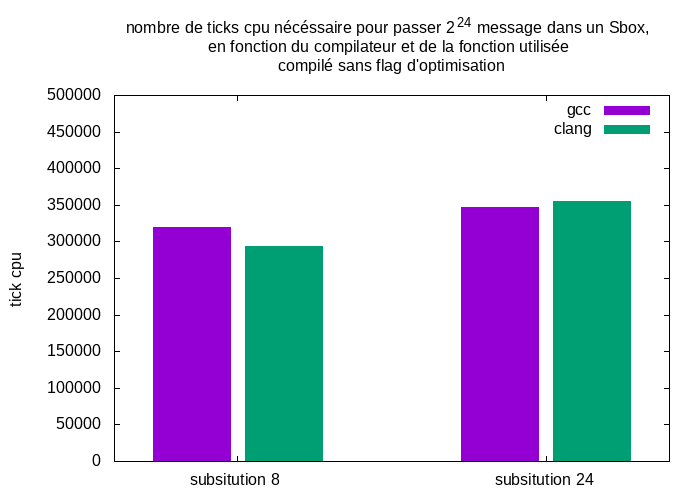
\includegraphics[width=12cm]{../src/benchmarks/substitution/img/substitution.png} \\ \\ \\
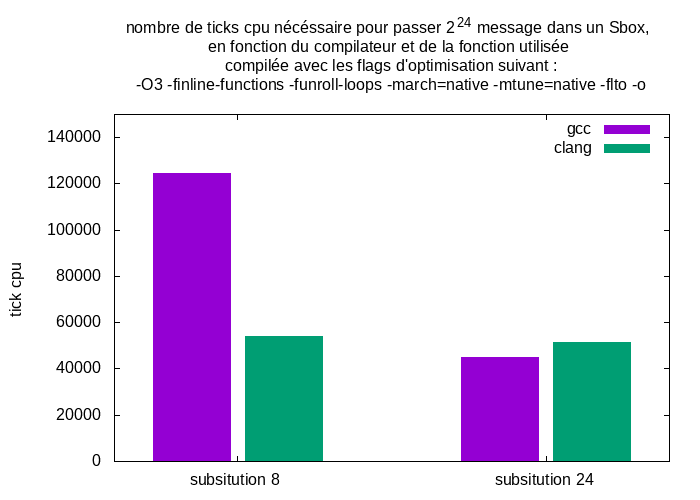
\includegraphics[width=12cm]{../src/benchmarks/substitution/img/substitution_opti.png}

\paragraph{} Chaque fonction a été testé avec et sans flag d'optimisation et avec GCC ou Clang. 
Il apparaît sur ces 2 graphiques que Clang semble plus performant que gcc. 
Aussi, la fonction substitution8 semble plus performante que substitution24  sans flag d'optimisation.
Lorsque l'on compare les 2 fonctions compilées avec des flags d'optimisations et avec clang, les résultats sont assez similaires mais substitution24 semble souvent plus rapide 

\section{ Permutation } 

\begin{lstlisting}
    u32_t pboxPermutation( u32_t m ){
        static const u32_t pbox[24] = {
            0,4,8,12,16,20,1,5,9,13,17,21,
            2,6,10,14,18,22,3,7,11,15,19,23
        };

        u32_t result = 0;
        for ( int i = 23; i >= 0; i-- )
        { 
            result <<= 1;
            if ( m & (1 << pbox[i]) )
                result |= 1;        
        }
        return result;

    }
\end{lstlisting}

\begin{lstlisting}
    u32_t magicPermutation( u32_t m ){
        u32_t r = 0x120c0600; //magic number 
        u32_t t = 0;
        for(u8_t j = 0; j < 24; j++  ) {
            // printf("r %d : %d %d \n", i, j,  (r & 255) );
            t |= ( ( m >> j ) & 1 ) << ( r & 255 );
            r = ( (r + 1) >> 8 ) | ( (r + 1) << (32 - 8) );   
        }
        return t;

    }
\end{lstlisting}

\paragraph{} la première fonction, pboxPermutation, est une permutation assez basique. 
Elle reçoit un message de 24 bits et va placer chaque bit du message à une place précise dans un variable résultat.
La deuxième fonction prend aussi un message de 24 bits en entrée, mais elle va utiliser un nombre magique, 
qui est en réalité un nombre particulier que l'on peut calculer en analysant le box. Pour chaque bit; 
la fonction va s'appuyer sur ce nombre magique pour effectuer le bon décalage et effectuer une opération pour modifier le nombre magique.

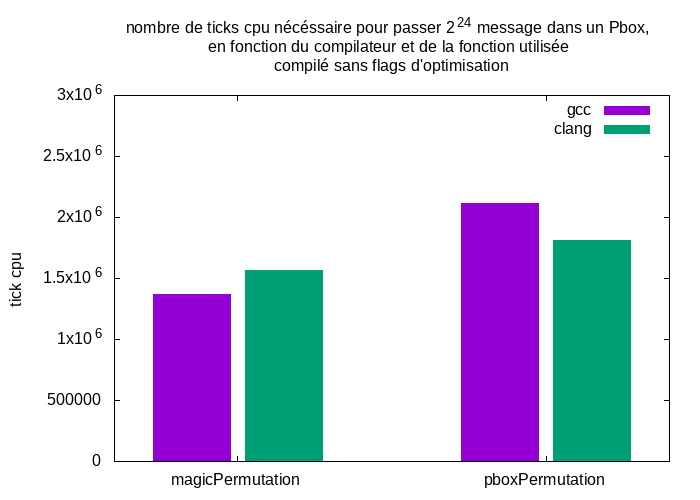
\includegraphics[width=12cm]{../src/benchmarks/permutation/img/permutation.png} \\ 
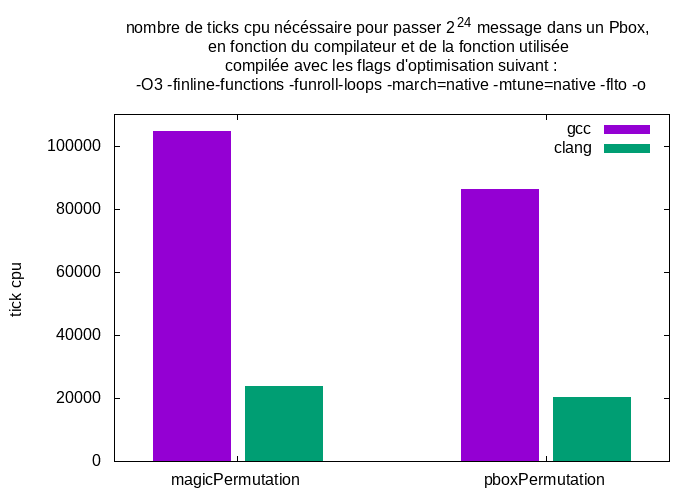
\includegraphics[width=12cm]{../src/benchmarks/permutation/img/permutation_opti.png}

\paragraph{} Chaque fonction a été testé avec et sans flag d'optimisation et avec GCC ou Clang. 
En premier lieu, la fonction magic permutation semble bien plus performante que la pboxPermutation si on regarde le graphique sans flag d'optimisation.
Cependant, lorsque les flags d'optimisations sont ajoutés, pboxPermutation compilées avec clang semble légèrement plus rapide que magicPermutation compilées aussi avec clang.
Et du coté de gcc, les résultats sont entre 4 et 5 fois plus lents ce qui conforte dans l'idée d'utiliser clang.

\section{ Key Scheduling } 


\begin{lstlisting}
    u32_t * keySchedulingOpt( u32_t key, u32_t * keys_24 ){

        static const u8_t sbox[16] = {
            0x0c,0x05,0x06,0x0b,0x09,0x00,0x0a,0x0d,
            0x03,0x0e,0x0f,0x08,0x04,0x07,0x01,0x02
        };
    
        
        u128_t cache = ((( ~((u128_t) 0)) << 48 ) >> 48) ;
        // u128_t cache = (u128_t) 10000000 ;
        u128_t mainKey = ((u128_t) key) << 56 ;
        u128_t K = mainKey;
    
        keys_24[ 0 ] = (K >> 16) & 0xffffff;
        
        for(int i = 1; i < 11; i++){
            K =  ( K << 61 | K >> 19 )  & cache;
            ((u8_t *)&K)[9] = (sbox[ ((u8_t *)&K)[9] >> 4] << 4) |  \
                ( 0x0f & ((u8_t *)&K)[9] ) ; 

            K = (((u128_t)(((K >> 15) ^ ((u128_t)i) ) << 15 )) | \
                ( K & ((u128_t)0b00000111111111111111) ))  & cache;
            //
            keys_24[ i ] = (K >> 16) & 0xffffff;
        }
    
    
        return keys_24;
    }
\end{lstlisting}
\newpage
\begin{lstlisting}
    u32_t * keyScheduling( u32_t key, u32_t * keys_24 ){

        static const u32_t pbox[24] = {
            0,6,12,18,1,7,13,19,2,8,14,20,
            3,9,15,21,4,10,16,22,5,11,17,23
        };

    
    
        u128_t cache = ((( ~((u128_t) 0)) << 48 ) >> 48) ;
        u128_t mainKey = ((u128_t) key) << 56 ;
        u128_t K = mainKey;
        keys_24[ 0 ] = (K >> 16) & 0xffffff;
        for(int i = 1; i < 11; i++){
            K =  ( K << 61 | K >> 19 ) & cache;
            K = ( (((u128_t) sbox[ K >> 76 ]) << 76 ) | \ 
                ( K & ~((u128_t) 0b1111 << 76) ) ) ;
            K = (( (((K >> 15) & 31 ) ^ (i) ) << 15 ) | \ 
                ( K & ~((u128_t)0b11111000000000000000) ) ) & cache;;
    
       
            keys_24[ i ] = (K >> 16) & 0xffffff;
        }
    
        return keys_24;
    }
\end{lstlisting}

\paragraph{} Les 2 fonctions de key scheduling sont très similaires et ne different que d'une ligne. 
La différence réside dans la gestion de la substitution.

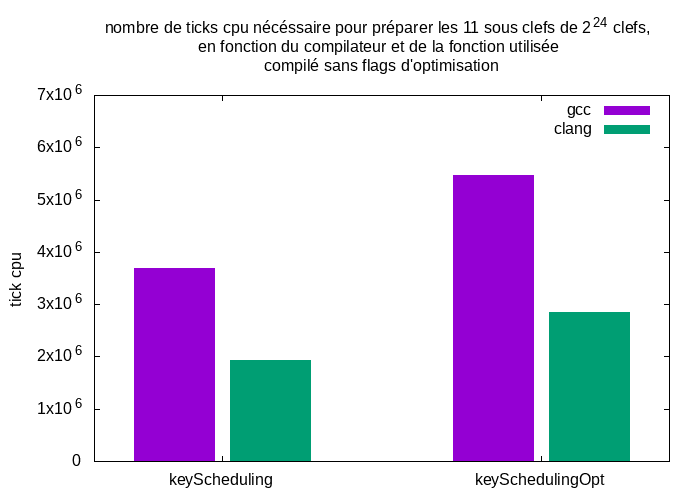
\includegraphics[width=12cm]{../src/benchmarks/keyScheduling/img/keyScheduling.png} \\ 
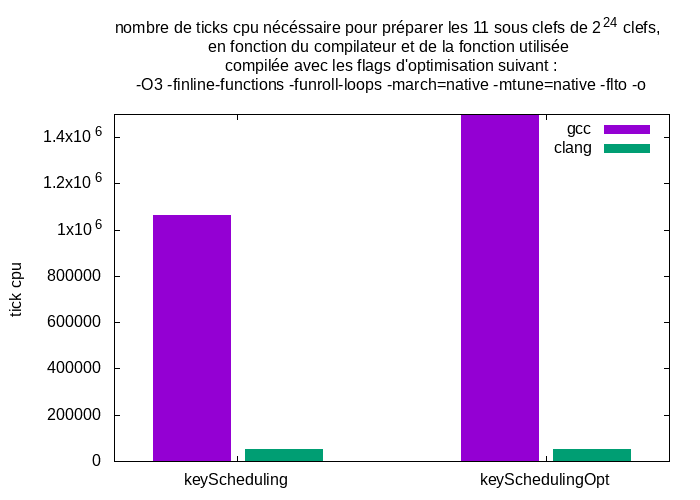
\includegraphics[width=12cm]{../src/benchmarks/keyScheduling/img/keyScheduling_opti.png}

\paragraph{} Chaque fonction a été testé avec et sans flag d'optimisation et avec GCC ou Clang. 
Les résultats ne sont pas très surprenants, clang est bien plus performant que gcc surtout avec les flags d'optimisation.
Les 2 versions compilées avec Clang semblent assez  similaires en matière de performance, avec un léger avantage pour la fonction key Scheduling
\chapter{Résultats} 
\section{ Performance globale } 
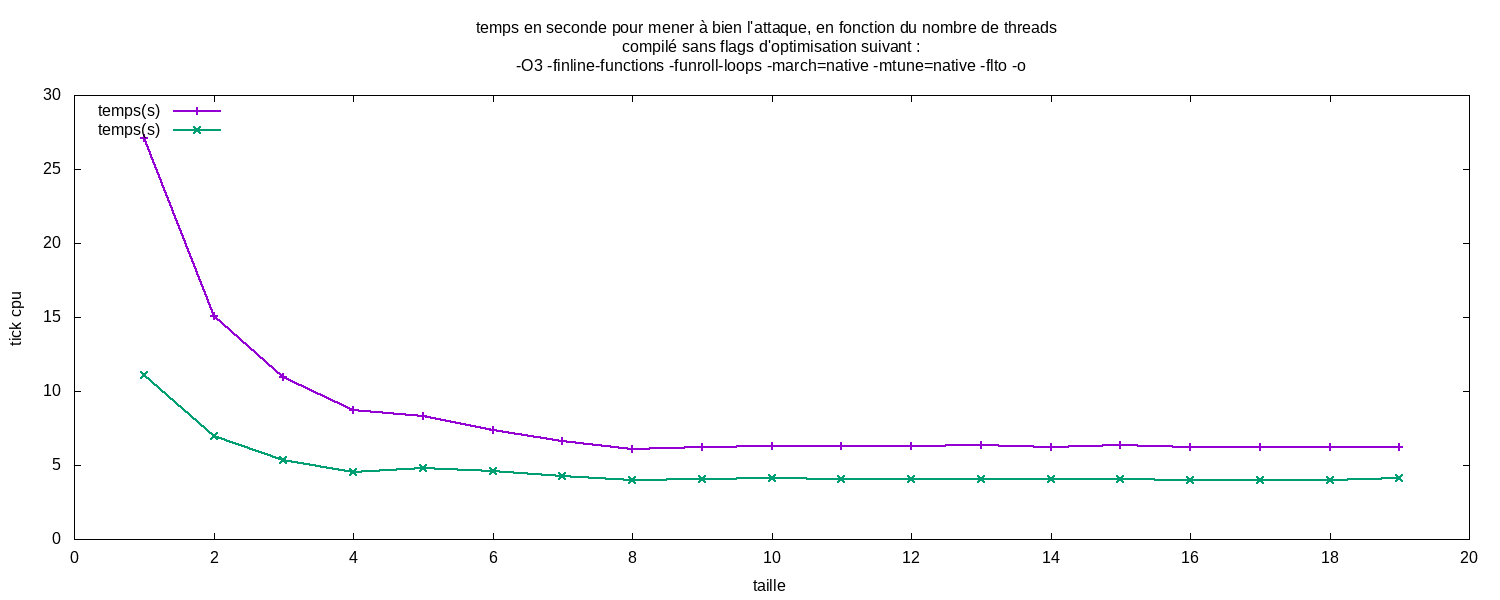
\includegraphics[width=15cm]{../src/benchmarks/attack/img/attack.png}

\paragraph{} 
Cette attaque a été performé sur un CPU intel i7 Core™ i7-4750HQ CPU @ 2.00GHz avec 4 coeurs et 8 threads.  
L'attaque effectuée avec un thread prend 27 secondes avec GCC et 11 avec Clang.
En augmentant le nombre de thread, on divise la tache. On remarque que le pic le plus bas, 
3.9 secondes se trouvent à 8 threads ce qui correspond au nombre du thread du cpu. 
Augmenter le le nombre de thread ne diminue pas plus le temps, voir l'augmente.

\section{ Complexité } 
Pour effectuer cette attaque, il a été nécessaire d'utiliser 2 tableaux de taille $2^{24} * 32bits$ pour stocker les clefs, 
et 2 tableaux de taille $2^{24} * 64bits$ pour stocker les chiffés et déchiffrés. On y ajoute aussi un tableau contenant les sous clef de taille  $11 * 32bits$.
On obtient donc une complexité en mémoire de : $2^{24} * 64 * 2 + 2^{24} * 32 * 2+ 11 * 32 => 2^{32} $ 
\\ ce qui équivaut à $2^{32}$ octets, et 512 Mo   \newline
La complexité en temps est de $4 * 2^{24}$ car on va venir chiffés 2 messages et déchiffrés 2 chiffrés $2^{24}$ fois.

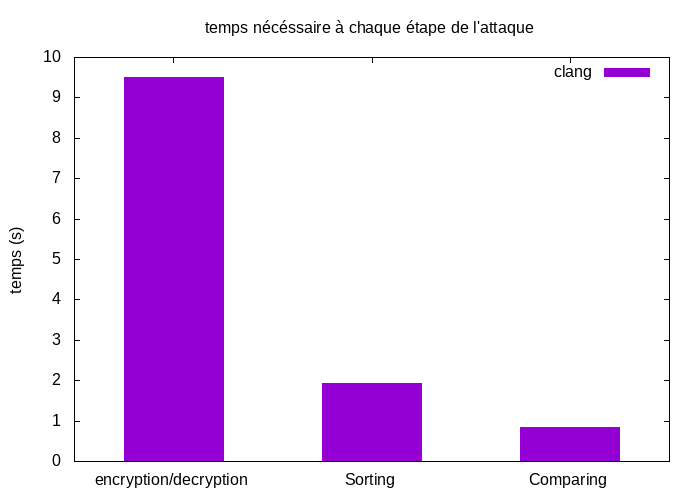
\includegraphics[width=12cm]{../src/benchmarks/attack/img/parts.png}


\paragraph{} 
La majeure partie de l'attaque et s'effectue sur le chiffrage et le déchiffrage des messages, d'où l'importance d'optimiser cette partie.
La section du tri dure 2 secondes, mais elle est divisée par 2 dès que l'on utilise plus d'un thread. 

\section{ Améliorations possibles } 
\paragraph{} 
Il reste beaucoup d'amélioration à faire à cette attaque que je n'ai pas eu le temps d'implémenter. 
Tout d'abord, il est possible d'implémenter le tris RADIX, un tris parallélisable  utilisé pour ordonner des éléments identifiés par une clef unique, ce qui correspond à notre cas.
Il est surement aussi possible d'optimiser le passage dans la Sbox et la Pbox, en s'appuyant sur la vectorisation des données, 
(bien que je suspecte clang de déja le faire au vu de ses performances.)


\end{document}
